\documentclass[addpoints]{exam}

\usepackage{amsmath,enumitem,wrapfig,physics}
\usepackage{tikz}

\newcommand{\StudentName}{Sabarno Saha - 22MS037}
\newcommand{\AssignmentName}{Waves and Optics }

\pagestyle{headandfoot}
\runningheadrule
\runningheader{PH2101}{\StudentName}{\AssignmentName}
\firstpagefooter{}{}{\thepage}
\runningfooter{}{}{\thepage}

\printanswers


\begin{document}


\par\textbf{IISER Kolkata} \hfill \textbf{Assignment 1}
\vspace{3pt}
\hrule
\vspace{3pt}
\begin{center}
        \LARGE{\textbf{PH2101 : Waves and Optics}}
\end{center}
\vspace{3pt}

\hrule
\vspace{4pt}
\textbf{Sabarno Saha}, \textbf{22MS037}\hfill \today

\vspace{20pt}

\bigskip

\begin{questions}

\question \textbf{ Question 1}
Consider a spring-mass oscillator of time period T as shown in the figure below. There is a wall $\frac{A}{2}$ distance to the right from the equilibrium position of the oscillator.
\begin{center}
    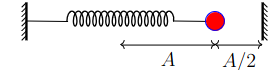
\includegraphics{q1.png}
\end{center}
The oscillator is given an initial displacement A towards the left and released from the rest.
Considering all collisions to be elastic, what is the time period of the oscillator?
\begin{solution}\\
 The general solution is given by 
 \begin{align*}
     x(t) &= A \sin(\omega t+ \phi) 
 \end{align*}
 We have the time period to be T thus $\omega = \frac{2\pi}{T}$. Since the collision is elastic the energy and momentum is conserved and as a result the only effect it has is 
 in the reduction of the time period. The collision being elastic just effectively reverses the velocity. As a result this just changes the phase of the system that what would 
 have been at a normal non-truncated SHM at that time.\\
 Then we know that the motion between the equilibrium position and the leftmost extreme and back takes $\frac{T}{2}$ to accomplish. The rest of the time is found out as t'.\\
 The half of the oscillation is unrestricted and thus takes time $\frac{T}{2}$. Also since the motion starts from the equilibrium position $\phi =0$. Let t be the time it takes to go from 
 the equilibrium position to the wall at $\frac{A}{2}$. Thus the time period is given by $T' = \frac{T}{2} + 2t$ where t is given by \\
 \begin{align*}
      &\frac{A}{2}  = A \sin(\omega t) \\
      \Rightarrow & \frac{1}{2} = \sin(\omega t)\\
      \Rightarrow & \omega t = \sin^{-1}\left(\frac{1}{2}\right) = \frac{\pi}{6} \\
      \Rightarrow & \frac{2\pi t}{T} = \frac{\pi}{6}\\
      \Rightarrow & t = \frac{T}{12}\\
 \end{align*}
\begin{align*}
      & T' = \frac{T}{2} + 2t \\
      \Rightarrow & T' = \frac{2T}{3}
 \end{align*} 
 Thus the total time period comes out to be  
 \begin{center}
     \fbox{$T' =\frac{2T}{3}$}
 \end{center}
\end{solution}

\question \textbf{ Question 2}
For an oscillator $\omega = \pm \omega_0$. If it started with $x(0)=A$ and $\Dot{x}(0) = \frac{\omega_0 A}{2}$, then find $x(t)$\\
Can you solve the problem using only $Ae^{i\omega_0 t}$? Why not?
\begin{solution}
 The general solution is given by 
 \begin{align*}
     x(t) &= C_1 \sin(\omega t ) + C_2 cos(\omega t)\\
     &= W\sin(\omega t +\phi)
 \end{align*}
 The boundary conditions give us 
 \begin{align*}
     & x(0) = C_2\cos(0) =A\\
     \Rightarrow & C_2=A \\
     &\Dot{x}(t) = C \omega_0 \cos(\omega t) - \omega_0 A \sin(\omega t)\\
     \Rightarrow &\Dot{x}(0) = C \omega_0 \cos(0) = \frac{\omega_0 A}{2}\\
     \Rightarrow &C_1 = \frac{A}{2}
 \end{align*}
 We can now find the phase difference by making the the coefficients of $\cos(\omega t)$ and $\sin(\omega t)$, $\sin(\phi)$ and $\cos(\phi)$ respectively.
 \begin{align*}
     &x(t) = \frac{A}{2}\sin(\omega_0 t) + A\cos(\omega_0 t)\\
     \Rightarrow & x(t) = \sqrt{A^2 + \frac{A^2}{4}} \left( \cfrac{A/2}{\sqrt{A^2 + \frac{A^2}{4}}}\sin(\omega_0 t) + \cfrac{A}{\sqrt{A^2 + \frac{A^2}{4}}}\cos(\omega_0 t)\right)\\
     \Rightarrow & x(t) = \frac{\sqrt{5A}}{2} \left( \cfrac{A/2}{\frac{\sqrt{5A}}{2}}\sin(\omega_0 t) + \cfrac{A}{\frac{\sqrt{5A}}{2}}\cos(\omega_0 t)\right)
 \end{align*}
 Let us define $\cos(\phi)$ and $\sin(\phi)$ as follows: 
 \begin{align*}
     \cos(\phi) &= \cfrac{A/2}{\frac{\sqrt{5A}}{2}}\\
     \sin(\phi) &= \cfrac{A}{\frac{\sqrt{5A}}{2}}
 \end{align*}
 We thus have $\tan (\phi) = \frac{A}{A/2} = 2$. Thus we have $\phi = \arctan(2)$
 \begin{align*}
     &x(t) = \frac{\sqrt{5A}}{2} \left( \cfrac{A/2}{\frac{\sqrt{5A}}{2}}\sin(\omega_0 t) + \cfrac{A}{\frac{\sqrt{5A}}{2}}\cos(\omega_0 t)\right)\\
     \Rightarrow & x(t) = \frac{\sqrt{5A}}{2}\sin\left(\omega_0t + \arctan(2)\right)
 \end{align*}
 \begin{center}
 \fbox{$x(t) = \frac{\sqrt{5A}}{2}\sin\left(\omega_0t + \arctan(2)\right)$}\\
 \end{center} 
 No we cannot only solve this using $Ae^{i\omega_0 t}$ because on differentiating and putting t=0 in the equation we get $i=\frac{1}{2}$ which is a mathematical absurdity. 
 Also physically this does not make sense as the IVP does make this a real Equation of motion as plugging in the initial value still keeps the amplitude a complex number.
\end{solution}
\question \textbf{ Question 3}
Consider the spring-mass system given below:
\begin{center}
    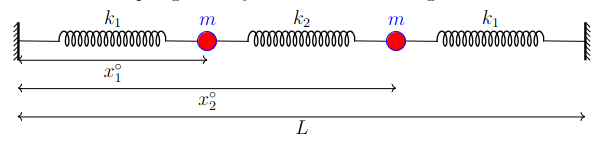
\includegraphics[width = 5 in]{q3.png}
\end{center}
\begin{enumerate}
    \item[a)] Find the equilibrium positions($x_1^o$ and $x_2^o$). Assume the equilibrium length of the spring $a_o$ to be $\frac{L}{10}$.
\end{enumerate}
\begin{solution}
    In the equilibrium position the force exerted by the middle and left springs on block $m_1$ are equal. The force due to the left spring on $m_1$ is 
    $F_l = -k_1(x^o_1 - a_o)$ and the force due to the middle spring on $m_1$ is $F_m = -k_2(x_2^o-x_1^o-a_o)$. Then we equate them
    \begin{align*}
        &F_l = F_m\\ 
        \Rightarrow & -k_1(x^o_1 - a_o) = -k_2(x_2^o-x_1^o-a_o)\\
        \Rightarrow & k_1(x^o_1 - a_o) = k_2(x_2^o-x_1^o-a_o) \\ 
        \Rightarrow & k_1x^o_1 - k_1a_o = k_2x_2^o-k_2x_1^o-k_2a_o \\
        \Rightarrow & (k_1+k_2)x_1^o-k_2 x_2^o = a_o(k_1-k2)
    \end{align*}
    We have from the diagram itself that $x_1^o + x_2^o = L\cdots (*)$.This equation is true because the system is symmetric about the $k_2$ spring.We also have 
    $a_0 =\frac{L}{10}$. We then multiply $(*)$ with $k_2$ to get $k_2x_1^o + k_2x_2^o = k_2L$ and then solve the system of equations.
    \begin{align}
        &(k_1+k_2)x_1^o-k_2 x_2^o = \frac{L}{10}(k_1-k_2)\\ 
        &k_2x_1^o + k_2x_2^o = k_2L 
    \end{align}
    Adding (2) and (1) we get 
    \begin{align*}
        &x_1^o(k_1+2k_2) = \frac{L}{10}(k_1-k_2) + k_2 L \\ 
        \Rightarrow & x_1^o = \frac{L}{10}\left(\frac{k_1+9k_2}{k_1+2k_2}\right)
    \end{align*}
    Then putting this value of $x_1^o$ in $(*)$ we have 
    \begin{align*}
        &x_2^o = L - \frac{L}{10}\left(\frac{k_1+9k_2}{k_1+2k_2}\right)\\ 
        \Rightarrow &  x_2^o = \frac{L}{10}\left(\frac{9k_1+11k_2}{k_1+2k_2}\right)
    \end{align*}
    Thus we have the equilibrium lengths to be
    \begin{center}
        \fbox{$x_1^o = \frac{L}{10}\left(\frac{k_1+9k_2}{k_1+2k_2}\right)$} \\
        \fbox{$x_2^o = \frac{L}{10}\left(\frac{9k_1+11k_2}{k_1+2k_2}\right)$}
    \end{center} 
    
\end{solution}


\textbf{ Question 3(b)}
Assuming unequal masses $m_1$ and $m_2$ and $k_1 = k_2 =k$, find the longitudinal normal mode frequencies.

\begin{solution}
    Let us move $m_1$ by $x_1$ and $m_2$ by $x_2$ both towards the right. Then we have two equations of motion for both of the masses
    \begin{align}
        &m_1\ddot{x_1} = -kx_1 -k(x_1-x_2)\nonumber\\
       \Rightarrow & m_1\ddot{x_1} = -2kx_1+kx_2)\\ 
        & m_2\ddot{x_2} = -kx_2 -k(x_2-x_1)\nonumber\\ 
       \Rightarrow & m_2\ddot{x_2} = -2kx_2 + kx_1
    \end{align}
    Putting test solutions $x_1 = Ae^{i\omega t}$ and $x_2=Be^{i\omega t}$ and eliminating $e^{i\omega t}$ from both sides we get
    \begin{align*}
        &(m_1\omega^2 - 2k)A + kB = 0 \\ 
        &(m_1\omega^2 - 2k)B + kA = 0
    \end{align*}
    Writing in matrix form we have the a matrix equation of the form $Ax=0$. Here we are looking for a non trivial solution thus the determinant of A has to be 0.
    \begin{align*}
        \begin{pmatrix}
            m_{1} \omega ^{2} -2k & k\\
            k & m_{1} \omega ^{2} -2k
        \end{pmatrix}  
        \begin{pmatrix}
            A\\
            B
        \end{pmatrix} = 
        \begin{pmatrix}
        0\\
        0
        \end{pmatrix}
    \end{align*}
    \begin{align*}
       \begin{vmatrix}
            m_{1} \omega ^{2} -2k & k\\
            k & m_{1} \omega ^{2} -2k
        \end{vmatrix}= 0
    \end{align*}
    \begin{align*}
        &(m_1\omega^2-2k)(m_2\omega^2 - 2k) - k^2 = 0 \\ 
        \Rightarrow & m_1m_2\omega^4 -2k\omega^2(m_1+m_2) + 3k^2 = 0 \\ 
        \Rightarrow & \omega^2 = \frac{2k(m_1+m_2) \pm \sqrt{4k^2(m_1+m_2)^2 - 12k^2m_1m_2}}{2m_1m_2} \\ 
        \Rightarrow & \omega^2 = \frac{k(m_1+m_2) \pm\ k\sqrt{m_1^2+m_2^2 - m_1m_2}}{m_1m_2}\\
        \Rightarrow & \omega = \pm \sqrt{\frac{k(m_1+m_2) \pm k\sqrt{m_1^2+m_2^2 - m_1m_2}}{m_1m_2}}
    \end{align*}
    Thus we have found the normal mode frequencies for a coupled spring mass system with different masses
\end{solution}


\textbf{ Question 5}
For longitudinal modes, assuming equal masses $m_1$ = $m_2$ (you may start from the
known solutions), find the $x_1(t)$ and $x_2(t)$ for motion starting from the rest with an
initial displacement $x_1(0) = A$ and $x_2(0) = \frac{A}{2}$?
\begin{solution}
    Again making the normal mode displacements but keeping the mass same this time while keeping the spring constants different we get the equations
    \begin{align}
        &m\ddot{x_1} = -k_1x_1 -k_2(x_1-x_2)\nonumber\\
       \Rightarrow & m_1\ddot{x_1} = -x_1(k_1+k_2) + k_2x_2\\ 
        & m\ddot{x_2} = -k_1x_2 -k_2(x_2-x_1)\nonumber\\ 
       \Rightarrow & m_2\ddot{x_2} = -k_1(x_1+x_2) + k_2x_1
    \end{align}
    Thus we can write as SHMs by algeabraic manipulation
    \begin{align*}
        m(\ddot{x_1^2}+\ddot{x_2^2}) = -k_1(x_1+x_2) \cdots (5)+(6)\\ 
        m(\ddot{x_1^2}+\ddot{x_2^2}) = -(k_1+2k_2)(x_1-x_2) \cdots (5)-(6)
    \end{align*}
    Thus they are second order differential equations with the cosine and sine functions. On differentiating and putting 0 in place of t only the coefficient of the original sine terms 
    remain. And since the motion starts from rest, the coefficients of the original sin terms go to 0.
    \begin{align}
        x_1 + x_2 = A_1 \cos(\omega_+t) ~\text{ where } \omega_+ = \pm\sqrt{\frac{k_1}{m}}\\ 
        x_1 - x_2 = A_2 \cos(\omega_-t) ~\text{ where } \omega_- = \pm\sqrt{\frac{k_1+2k_2}{m}}
    \end{align}
    Putting in boundary values given to us we obtain $A_1=\frac{3A}{2}$ and $A_2 = \frac{A}{2}$. On doing (7) + (8) we get function $x_1(t)$ and on doing (7) - (8) we get the function
    $x_2(t)$ we get 
    \begin{align*}
        x_1(t) = \frac{A}{4}\left(3\cos(\omega_+t) + \cos(\omega_-t)\right)\\ 
        x_2(t) = \frac{A}{4}\left(3\cos(\omega_+t) - \cos(\omega_-t)\right)
    \end{align*}
\end{solution}

\question \textbf{ Question 4}
Find the normal modes (frequencies and ratios of amplitude) for the transverse oscillation of
the following system:\\
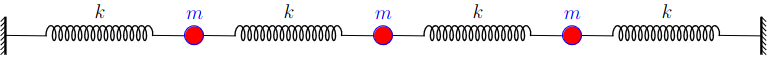
\includegraphics[width=5.0in]{q4.png}

\begin{solution}
    Let us displace the first mass by $y_1$ the second by $y_2$ and the third by $y_3$.\\
    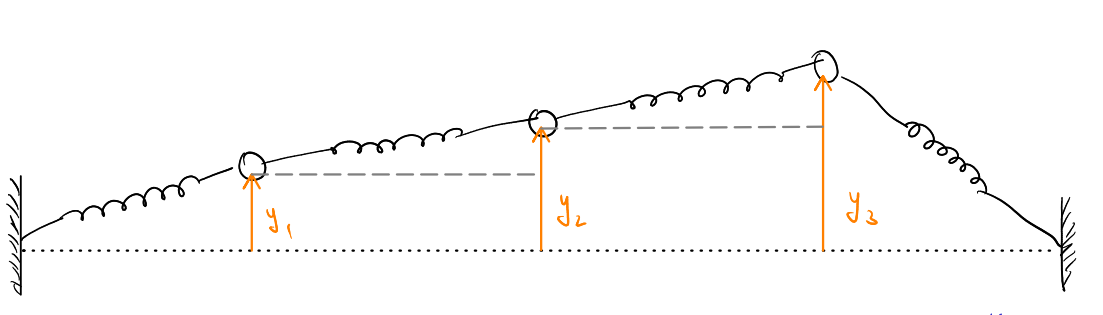
\includegraphics[width = 5.0 in]{q4ans.png}\\ 
    We assume that the displacements are small and let $T = k(a-a_0)$ where a is the equilibrium length of the spring when kept in a straight line and $a_0$ is the natural length of a spring\\ 
    \begin{align*}
        &m\ddot{y_1} = -\frac{Ty_1}{a} + \frac{T(y_2-y_1)}{a}\\ 
        \Rightarrow & \ddot{y_1} = -\frac{2Ty_1}{ma} + \frac{Ty_2}{ma}\\
        &m\ddot{y_2} = -\frac{T(y_2-y_1)}{a} + \frac{T(y_3-y_2)}{a}\\ 
        \Rightarrow & \ddot{y_1} = \frac{Ty_1}{ma} - \frac{2Ty_2}{ma} + \frac{Ty_3}{ma}\\
        &m\ddot{y_3} = -\frac{(Ty_3}{a} - \frac{T(y_3-y_2)}{a}\\ 
        \Rightarrow & \ddot{y_1} = -\frac{2Ty_3}{ma} + \frac{Ty_2}{ma}
    \end{align*}
    Then let $\frac{T}{ma} = \omega_0^2$ and as previously done use guessed solutions $y_1 = Ae^{i\omega t},  y_2 = Be^{i\omega t},y_3 = Ce^{i\omega t}$. 
    \begin{align}
         \ddot{y_1} = -2\omega_0^2y_1 + \omega_0^2y_2\\
         \ddot{y_2} = \omega_0^2y_1 - 2\omega_0^2y_2 + \omega_0^2y_3\\
         \ddot{y_3} = -2\omega_0^2y_1 + \omega_0^2y_2
    \end{align}
    Putting these in the above equations and cancelling the $e^{i\omega t}$ terms on both sides for all the equations we get the matrix equation ;
    \begin{align*}
        \begin{pmatrix}
            \omega ^{2} -2\omega _{0}^{2} & \omega _{0}^{2} & 0\\
            \omega _{0}^{2} & \omega ^{2} -2\omega _{0}^{2} & \omega _{0}^{2}\\
            1 & \omega _{0}^{2} & \omega ^{2} -2\omega _{0}^{2}
        \end{pmatrix} 
        \begin{pmatrix}
            A\\
            B\\
            C
        \end{pmatrix}=
        \begin{pmatrix}
            0\\
            0\\
            0
        \end{pmatrix}
        \\ \\ \\
        \begin{vmatrix}
            \omega ^{2} -2\omega _{0}^{2} & \omega _{0}^{2} & 0\\
            \omega _{0}^{2} & \omega ^{2} -2\omega _{0}^{2} & \omega _{0}^{2}\\
            1 & \omega _{0}^{2} & \omega ^{2} -2\omega _{0}^{2}
        \end{vmatrix} =0
    \end{align*}
    Opening the determinant and simplifying we get 
    \begin{align*}
        &(\omega^2-2\omega_0^2)[(\omega^2-2\omega_0^2)^2-2\omega_0^4] = 0\\ 
        \Rightarrow & (\omega^2-2\omega_0^2)=0 \text{  or  } [(\omega^2-2\omega_0^2)^2-2\omega_0^4] = 0\\ 
        \Rightarrow & \omega=\pm\sqrt{2}\omega_0 \text{  or  } \omega^2=\pm \sqrt{2\pm\sqrt{2}}\omega_0
    \end{align*}
    Now putting the values in the matrix and then getting their corresponding equations we get three  :
    \textbf{Case 1: $\omega^2=2\omega_0^2$}\\ 
    \begin{enumerate}
        \item eqn (9) $B=0$
        \item eqn(10) $A+C=0$
    \end{enumerate}
        Solving gives us $A = -C$ and $B=0$\\ 
        \textbf{Case 2: $\omega^2=(2+\sqrt{2})\omega_0^2$}
\end{solution} 

\end{questions}
\end{document}
